\section{在实践中构建分组密码}

分组密码是密码学中的一个基本原语,许多其他系统都是基于它建立的。几乎所有在实践中使用的分组密码都使用了相同的基本框架,被称为\textbf{迭代密码 (iterated cipher)}范式。为了构建一个迭代分组密码,设计者需要做出以下两个抉择:
\begin{itemize}
	\item 首先,他需要选择一个简单的分组密码 $\mathcal{\hat E}:=(\hat E,\hat D)$,它本身显然是不安全的。我们称 $\mathcal{\hat E}$ 为\textbf{轮密码 (round cipher)}。
	\item 其次,他还需要选择一个简单(但不一定安全)的 PRG $G$,用来将密钥 $k$ 扩展为 $\mathcal{\hat E}$ 的 $d$ 个密钥 $k_1,\dots,k_d$。我们称 $G$ 为\textbf{密钥扩展函数 (key expansion function)}。
\end{itemize}
一旦做出这两个选择,迭代分组密码 $\mathcal{E}$ 就完全确定下来了。加密算法 $E(k,x)$ 的工作原理如下(另见图 \ref{fig:4-6}):

\begin{figure}
  \centering
  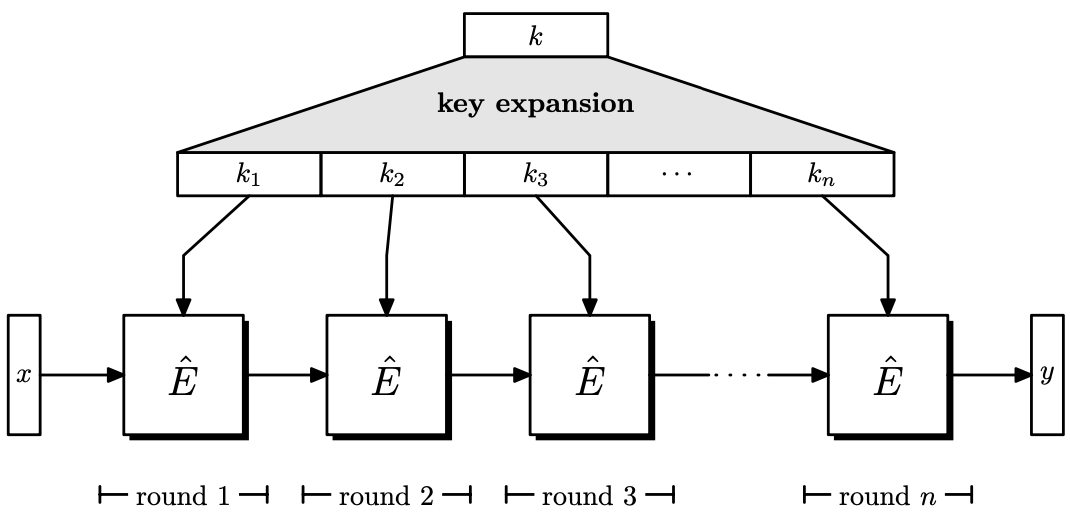
\includegraphics[width=0.7\linewidth]{figures/chapter4/fig6.png}
  \caption{现实世界中分组密码的加密}
  \label{fig:4-6}
\end{figure}

\begin{quote}
\begin{quote}
\begin{quote}
\begin{tcolorbox}[colframe=black,colback=white,boxrule=0.6pt,arc=0pt]
算法$E(k,x)$:

\vspace{5pt}

\begin{enumerate}
	\item \textbf{密钥扩展}:使用密钥扩展函数 $G$ 将 $\mathcal{E}$ 的密钥 $k$ 扩展为 $\mathcal{\hat E}$ 的 $d$ 个密钥:
	\[(k_1,\dots,k_d)\leftarrow G(k)\]
    \item \textbf{迭代}:对于 $i=1,2,\dots$,应用 $d$ 次 $\hat E(k_i,\cdot)$,即:
    \[y\leftarrow\hat{E}(k_d,\;\hat{E}(k_{d-1},\dots,\hat{E}(k_2,\;\hat{E}(k_1,\;x))\dots))\]
\end{enumerate}
\end{tcolorbox}
\end{quote}
\end{quote}
\end{quote}
每次应用 $\mathcal{\hat E}$ 称为一\textbf{轮 (round)},总轮数为 $d$。$k_1,\dots,k_d$ 被称为\textbf{轮密钥 (round keys)}。解密算法 $D(k, y)$ 与加密算法 $E(k,x)$ 基本相同,除了解密时轮密钥是被反向使用的。$D(k,y)$ 的定义如下:
\[
x\leftarrow\hat{D}(k_1,\hat{D}(k_2,\dots,\hat{D}(k_{d-1},\hat{D}(k_d,y))\dots))
\]
表 \ref{tab:4-1} 列出了一些常见的分组密码和它们的相关参数。我们将在下一节中介绍 DES 和 AES。

\begin{snote}[迭代是否能提供一个安全的分组密码?]
没有人知道。然而,启发式的证据表明,分组密码的安全性来自于对简单密码的多次迭代。但并非所有的轮密码都能发挥作用。例如,迭代一个这样的线性函数:
\[
\hat E(k,x)=k\cdot x\mod q
\]
无论多少次都不会生成一个安全的分组密码,因为 $\hat E$ 的迭代只会是另一个线性函数。目前还没有办法辨别哪些轮密码最终能产生安全的分组密码。此外,对于一个候选的轮密码 $\hat E$,我们也还没有严格的方法来衡量需要迭代它多少次才能生成一个安全的分组密码。我们知道的是,某些函数,比如线性函数,是完全不可能导出安全分组密码的。但是简单的非线性函数似乎在几次迭代后就能得到一个安全的分组密码。

密码学家面临的挑战是要想出一个快速的轮密码,它在几轮之内就能收敛为一个安全分组密码。看看表 \ref{tab:4-1},拿 AES-128 来说,它使用了一个很简单的轮密码,但只需要十轮就能够产生一个安全的分组密码,这种性能就十分理想。
\end{snote}

\begin{table}
\centering
\begin{tabular}{lcccc}
\hline
 &
  \begin{tabular}[c]{@{}c@{}}key size\\ (bits)\end{tabular} &
  \begin{tabular}[c]{@{}c@{}}block size\\ (bits)\end{tabular} &
  \begin{tabular}[c]{@{}c@{}}number of\\ rounds\end{tabular} &
  \begin{tabular}[c]{@{}c@{}}performance\footnotemark[1]\\ (MB/s)\end{tabular} \\ \hline
DES     & 56  & 64  & 16 & 80  \\
3DES    & 168 & 64  & 48 & 30  \\
AES-128 & 128 & 128 & 10 & 163 \\
AES-256 & 256 & 128 & 14 & 115 \\ \hline
\end{tabular}
\caption{分组密码示例}
\label{tab:4-1}
\end{table}

\footnotetext[1]{性能数字是使用 OpenSSL 1.0.1e 在 Intel(R) Xeon(R) CPU E5-2698 v3 @ 2.30GHz (Haswell) 处理器上运行获得的。}

\begin{snote}[注意事项。]
虽然本节解释了几种分组密码的内部工作原理,但它并没有教授如何设计新的分组密码。事实上,本节的主要收获之一是,读者不应自行设计分组密码,而应该始终使用这里描述的标准密码。分组密码的设计非同小可,需要经过多年的分析才能对某一具体方案产生充分信心。此外,读者甚至不应该自己实现分组密码,因为分组密码的实现往往容易受到计时攻击和功耗攻击,就如 \ref{subsec:4-3-2} 小节将要讨论的。使用诸如 OpenSSL 等密码库中免费提供的标准实现要安全得多。这些实现经历了多年来的反复分析,并已被多次加固以抵御各种攻击。
\end{snote}

\subsection{案例研究:DES}\label{subsec:4-2-1}

上世纪 70 年代,美国国家标准局 (National Bureau of Standards, NBS),即现在的美国国家标准技术研究所 (National Institute of Standards and Technology, NIST) 向社会公开征集加密方案。因应这一需求,IBM 开发了数据加密标准 (Data Encryption Standard, DES)。它于 1975 年在联邦公报上发表,并于 1977 年被采纳为``非机密"应用的加密标准。DES 算法单枪匹马地开启了密码分析领域,因为所有人都想破解它。自诞生以来,DES 经历了相当多的分析,也间接导致了许多分组密码分析工具的出现。

DES 的前身是 IBM 早期设计的一个分组密码,名为 Lucifer。Lucifer 的某些变体使用 $128$ 比特密钥对 $128$ 比特的分组进行操作。然而,国家标准局要求设计使用更短分组($64$ 比特)和更短密钥($56$ 比特)的分组密码。作为回应,IBM 团队设计了一个符合这些要求的密码,并在最终成为了 DES。将 DES 的密钥大小设定为 $56$ 比特在当时饱受批评。甚至有人猜测 DES 的这种弱设计是美国情报机构故意要求的。在接下来的章节中,我们还会看到将分组大小减少到 $64$ 比特也带来了许多问题。

由于密钥太短,DES 算法现在被认为是不安全的,不应该再被使用。然而,一个名为 3DES 的加强版 DES 在 1998 年被重新确立为美国国家标准。NIST 已经批准 3DES 供政府使用直至 2030 年。在 2002 年,DES 被一个更高效的分组密码标准所取代,即 AES,它使用 $128$ 比特(或更长)的密钥,并在 $128$ 比特的分组上运行。

\subsubsection{DES 算法}

DES 算法由一个简单的轮密码经 $16$ 次迭代组成。为了描述 DES,我们需要先介绍 DES 轮密码和 DES 密钥扩展函数。我们下面依次介绍它们。

\begin{snote}[费斯妥置换法。]
DES 的关键创新之一是由 IBM 的霍斯特·费斯妥 (Horst Feistel) 发明的费斯妥置换法 (Feistel Permutation),它能基于任意函数建立一个置换。令 $f:\mathcal{X}\to\mathcal{X}$ 是一个函数,我们按如下方法构建一个置换 $\pi:\mathcal{X}^2\to\mathcal{X}^2$(见图 \ref{fig:4-7}):
\[
\pi(x,y):=(y,\;x\oplus f(y))
\]
为了证明 $\pi$ 是一个双射,我们给出它的逆变换:
\[
\pi^{-1}(u,v)=(v\oplus f(u),\;u)
\]
映射 $\pi$ 被称为\textbf{费斯妥置换},它被用于构建 DES 轮密码。$n$ 个费斯妥置换的组合被称为 \textbf{$n$ 轮费斯妥网络 ($n$-round Feistel network)}。设计成费斯妥网络的分组密码被称为\textbf{费斯妥密码}。对于 DES 来说,函数 $f$ 需要 $32$ 比特输入,产生的映射 $\pi$ 对 $64$ 比特的分组进行操作。

需要注意的是,费斯妥逆置换 $\pi^{-1}$ 几乎与 $\pi$ 相同。因此,只用设计同一套硬件电路就能计算 $\pi^{-1}$ 和 $\pi$。这也意味着加密和解密电路也可以使用相同的硬件实现。
\end{snote}

\begin{figure}
  \centering
  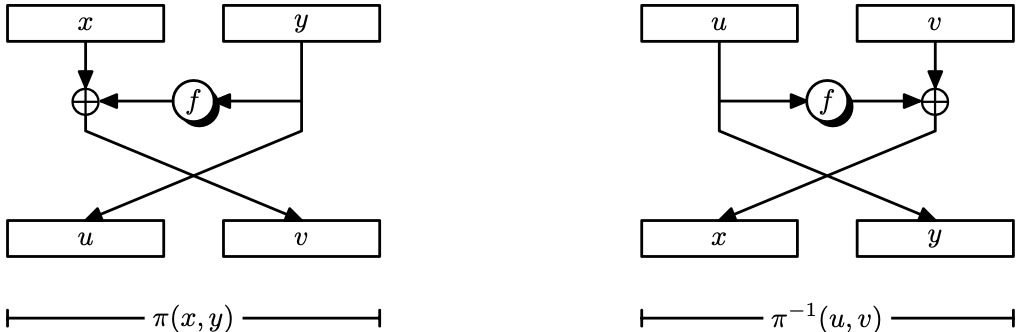
\includegraphics[width=0.7\linewidth]{figures/chapter4/fig7.png}
  \caption{费斯妥置换法}
  \label{fig:4-7}
\end{figure}

\begin{figure}[p!]
  \centering
  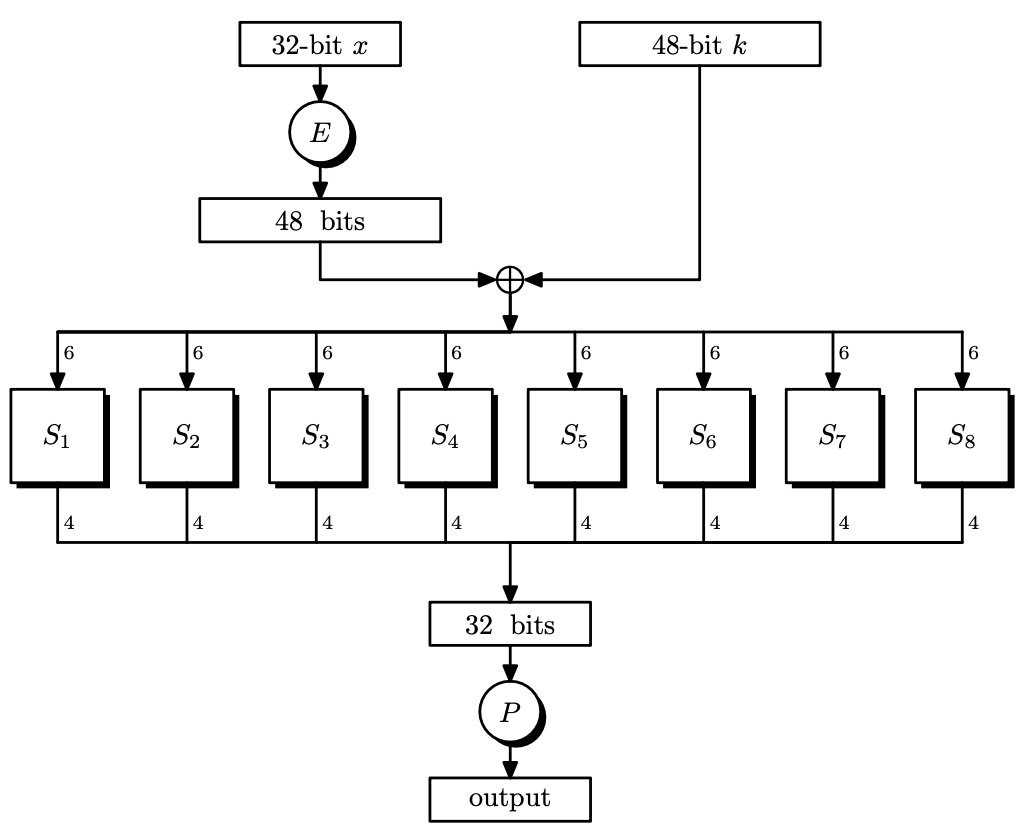
\includegraphics[width=0.85\linewidth]{figures/chapter4/fig8.png}
  \caption{DES的轮函数$F(k,x)$}
  \label{fig:4-8}
\end{figure}

\begin{snote}[DES 轮函数。]
DES 加密算法是一个 $16$ 轮费斯妥网络,每轮使用一个不同的函数 $f:\mathcal{X}\to\mathcal{X}$。在第 $i$ 轮中,函数 $f$ 的定义为:
\[
f(x):=F(k_i,x)
\]
其中,$k_i$ 是第 $i$ 轮的 $48$ 比特密钥,$F$ 是一个固定函数,称为 \textbf{DES 轮函数}。函数 $F$ 是 DES 算法的核心,如图 \ref{fig:4-8} 所示。$F$ 使用的几个辅助函数 $E$、$P$ 和 $S_1,\dots,S_8$ 定义如下:
\begin{itemize}
	\item 函数 $E$ 通过对输入比特的重新排列和复制,将 $32$ 比特输入扩展为 $48$ 比特输出。例如,$E$ 将输入的第 $1$ 比特映射到输出的第 $2$ 和第 $48$ 比特,将输入的第 $2$ 比特映射到输出的第 $3$ 比特,以此类推。
	\item 函数 $P$ 称为\textbf{混合置换 (mixing permutation)},它通过重新排列输入的比特,将 $32$ 比特输入映射到 $32$ 比特输出。例如,$P$ 将输入的第 $1$ 比特映射到输出的第 $9$ 比特,将输入的第 $2$ 比特映射到输出的第 $15$ 比特,以此类推。
	\item 函数 $S_1,\dots,S_8$ 称为 \textbf{S 盒 (S-boxes)}。每个 S 盒 $S_i$ 通过一个查找表将一个 $6$ 比特输入映射到一个 $4$ 比特输出。DES 标准列出了这 $8$ 张查找表,每张表中包含 $64$ 个条目。
\end{itemize}

\noindent
基于以上函数,DES 的轮函数 $F(k,x)$ 工作原理如下:

\vspace*{5pt}

\hspace*{5pt} 输入:$k\in\{0,1\}^{48}$ 和 $x\in\{0,1\}^{32}$\\
\hspace*{26pt} 输出:$y\in\{0,1\}^{32}$

\vspace*{5pt}

\hspace*{5pt} $F(k,x)$:\\
\hspace*{50pt} 计算 $t\leftarrow E(x)\oplus k\in\{0,1\}^{48}$\\
\hspace*{50pt} 将 $t$ 分成 $8$ 组,每组 $6$ 比特:$t:=t_1\,\Vert\,\cdots\,\Vert\,t_8$\\
\hspace*{50pt} 对于 $i=1,2,\dots,8$,令 $s_i\leftarrow S_i(t_i)$\\
\hspace*{50pt} 组合 $s\leftarrow s_1\,\Vert\,\cdots\,\Vert\,s_8\in\{0,1\}^{32}$\\
\hspace*{50pt} 计算 $y\leftarrow P(s)\in\{0,1\}^{32}$\\
\hspace*{50pt} 输出 $y$

\vspace*{5pt}

\noindent
除了 S 盒,DES 的轮密码完全由异或操作和比特置换组成。八个 S 盒是设计中唯一引入的非线性组件。在公开文献揭示了一种名为``差分密码分析"的强大攻击技术后,IBM 于 1994 年公布了设计 S 盒的标准。IBM 的这份报告清楚地表明,DES 的设计者早在 1973 年就已经了解了多年后才在公开文献中出现的这种攻击技术。他们在设计 DES 时加入了抵抗这种攻击的因素。下面这段话解释了对 S 盒设计标准保密的原因:
\begin{quote}
我们在设计 DES 时利用了某些密码分析技术的知识,其中最突出的是``差分密码分析"技术,这些技术在公开的文献中并不为人所知。在与美国国家安全局讨论后,我们认为如果披露设计思路,就会反过来揭示这种差分密码分析技术。这种技术非常强大,可以用来对付很多密码器,因此会削弱美国在密码学领域相对其他国家的竞争优势。
\end{quote}
一旦差分密码分析技术被公开,再保密 DES 的设计思路也就没太多意义了。由于 S 盒的重要性,我们下面列举了当初设计它的一些准则:
\begin{enumerate}
	\item 将 $6$ 比特输入映射到 $4$ 比特输出的查找表,是以 1974 年的技术能在单个芯片上做到的最大尺寸;
	\item S 盒的任何输出比特都不应该接近于输入比特的线性函数。也就是说,如果我们选择任何一个输出比特和 $6$ 个输入比特的任何一个子集,这个输出比特等于这些输入比特的异或结果的概率应该接近 $\frac{1}{2}$;
	\item 如果我们把输入的最左边和最右边的比特固定在一个 S 盒上,那么产生的 $4$ 比特到 $4$ 比特的函数是一个双射。特别地,这意味着每个 S 盒都是一个 $4$ 到 $1$ 的映射;
	\item 改变一个 S 盒的输入比特,至少会改变输出的两个比特;
	\item 对于 $x,y\in\{0,1\}^6$ 的 $64$ 种可能情况,令 $\Delta=x\oplus y\in\{0,1\}^6$,$S_i(x)\oplus S_i(y)$ 的结果是同一个值最多不能超过 $8$ 次。
\end{enumerate}
这些标准是为了使 DES 在 $56$ 比特密钥大小的限制下能尽可能地强大。现在我们已经知道,如果 S 盒是简单随机选出的,那么很有可能产生的 DES 密码是不安全的。特别是,可能只需要对挑战者进行几百万次查询,对手就可以恢复出秘钥。

除了 S 盒之外,混合置换 $P$ 也起着重要的作用。它确保 S 盒不总是在同一组 $6$ 比特上进行操作。同样,$P$ 也是根据一些标准决定的。如果 $P$ 是简单随机选出的,那么 DES 的安全性也将大打折扣。
\end{snote}

\begin{figure}
  \centering
  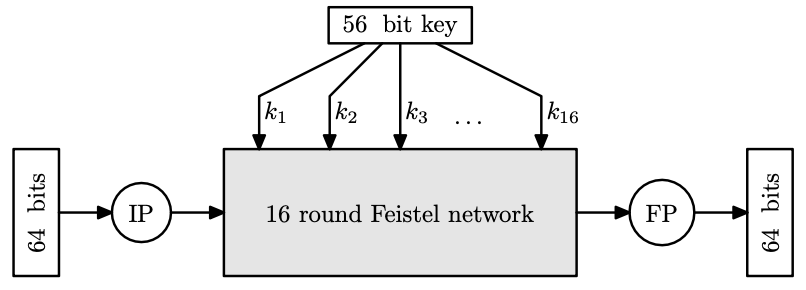
\includegraphics[width=0.6\linewidth]{figures/chapter4/fig9.png}
  \caption{完整的DES电路}
  \label{fig:4-9}
\end{figure}

\begin{snote}[密钥扩展函数。]
DES 的密钥扩展函数 $G$ 将 $56$ 比特的密钥 $k$ 作为输入,输出 $16$ 个密钥 $k_1,\dots,k_{16}$,每个 $48$ 比特长。每个密钥 $k_i$ 都由从 $56$ 比特密钥 $k$ 中选出的 $48$ 比特组成,每个 $k_i$ 使用 $k$ 中不同比特的子集。
\end{snote}

\begin{snote}[DES 算法。]
完整的 DES 算法架构如图 \ref{fig:4-9} 所示,它包括 DES 轮密码的 $16$ 次迭代,以及被称为 IP 和 FP 的初始和最后的置换排列。这些置换只是重新排列了 $64$ 比特的输入和输出,其中 FP 变换是 IP 变换的逆变换。

IP 和 FP 没有任何密码学意义,被包括在算法内的原因至今不明。由于比特置换在软件实现中很慢,但在硬件实现中却很快,一种理论认为,IP 和 FP 是为了故意减慢 DES 的软件实现而加入的。
\end{snote}

\subsection{对DES的穷举搜索:DES的挑战}\label{subsec:4-2-2}

回顾一下,对分组密码 $(E,D)$ 的穷举搜索攻击(\ref{subsubsec:4-1-1-2} 小节)指的是这样的攻击:给予对手少量的明文分组 $x_1,\dots,x_Q\in\mathcal{X}$ 和使用 $\mathcal{K}$ 中的密钥 $k$ 加密它们得到的密文分组 $y_1,\dots,y_Q$。对手尝试所有可能的 $\mathpzc{k}\in\mathcal{K}$,直至找到一个密钥 $k$,能够将给定的明文转化为给定的密文。如果给定的密文分组足够多,$k$ 就能够被对手唯一确定。

对于像 DES 和 AES-128 这样的分组密码,仅需三个分组就足以确保有唯一密钥能以较大概率将给定的明文分组映射到给定的密文分组。我们将在 \ref{subsec:4-7-2} 小节讨论理想密码及其特性时看到原因。现在我们只需知道,给定三个明文/密文分组对,攻击者就可以用穷举法找到秘钥 $k$。

在 1974 年设计 DES 时,对 $256$ 比特的密钥空间进行穷举搜索攻击被认为是不可行的。但随着计算机硬件的持续发展,人们渐渐发现 $56$ 比特的密钥远远不够。

为了证明对 DES 的穷举搜索是可行的,RSA 数据安全部设置了一连串的挑战,称为 \textbf{DES 挑战}。规则很简单:在一个预先宣布的日期,RSA 数据安全部公布了 DES 的三个输入/输出对。第一个找到相应密钥的小组就能赢得一万美元。为了使挑战更具娱乐性,挑战包含 $n$ 个 DES 输出 $y_1,y_2,\dots,y_n$,其中前三个输出 $y_1,y_2,y_3$ 是对下面这 $24$ 字节明文消息应用 DES 后得到的结果:

\begin{figure*}[h!]
  \centering
  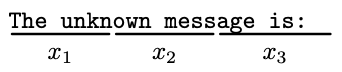
\includegraphics[width=0.3\linewidth]{figures/chapter4/fig-vac1.png}
\end{figure*}
它由 $3$ 个 DES 分组构成,每个分组为 $8$ 字节,也就是 $64$ 比特。目标是找到一个 DES 密钥,对于 $i=1,2,3$,该密钥能够将 $x_i$ 映射到 $y_i$。得到密钥后,挑战者就能够使用密钥来解密 $y_4,\dots,y_n$ 编码的秘密消息。

第一个挑战在 1997 年 1 月发布。DESCHALL 项目组用 96 天的时间解决了它。该团队在 78,000 名志愿者的帮助下使用众包搜索的方式进行破解,这些志愿者贡献了他们自己设备的闲置算力。找到秘钥的志愿者获得了 $40\%$ 的奖金。解密后大家得知,$y_4,\dots,y_n$ 对应的明文是``强大的密码学使世界更加安全。" (Strong cryptography makes the world a safer place.)

第二个挑战于 1998 年 1 月发布。\textbf{distributed.net} 项目组使用了类似的但规模更大的众包搜索,仅用时 41 天就解决了该挑战。

1998 年初,电子前沿基金会 (Electronic Frontiers Foundation, EFF) 与 Paul Kocher 签订合同,建造一台专门的设备来进行针对 DES 的穷举密钥搜索。这台机器被称为\textbf{DeepCrack},耗资 25 万美元,包含大约 1900 个专用 DES 芯片,装在六个柜子里。这些芯片并行工作,每个芯片在指定的密钥空间中搜索。当 RSA 数据安全部在 1998 年 7 月发布下一个挑战时,DeepCrack 在 56 小时内就解决了这个挑战,并轻松赢得了一万美元的奖金。这还不足以支付机器的成本,但足以说明 DES 存在致命问题。

最后的挑战是在 1999 年 1 月发布的。在 DeepCrack 和 \emph{distributed.net} 的共同努力下,它在 22 小时内就被破解了。这在 DES 的棺材板上钉上了最后一颗钉子,表明 $56$ 比特的密钥可以在短短几个小时内就被破解。

在这个故事的末尾,2007 年,\textsc{copacobana} 团队建立了一个由现成的 120 块 FPGA 板组成的集群,总成本约为 1 万美元。该集群可以在大约 12.8 天内搜索完整个 $2^{56}$ DES 密钥空间。

上述所有工作将我们导向一个共同的结论,那就是 $56$ 比特密钥太短了。目前的最小安全密钥长度是 $128$ 比特。

\subsubsection{穷举搜索对 AES-128 是否奏效?}

让我们把 DES 上的结论推广到 AES。虽然这些估计本身是不精确的,但它们在一定程度上说明了针对 AES 的穷举搜索的复杂性。AES 的密钥空间最小是 $2^{128}$。如果扫描一个 $2^{56}$ 的空间需要 22 小时,那么扫描一个 $2^{128}$ 大小的空间将需要:
\[
(22~{\rm hours})\times2^{128-56}\approx1.18\times10^{20}~{\rm years}
\]
即使计算速度和计算资源能提升十亿倍,即使 AES 计算比 DES 计算更快,所需的时间也远超人类的认知范围。因此,我们可以得出这样的结论:对 AES 进行暴力穷举式的搜索攻击是不现实的。然而,正如我们将在 \ref{sec:18-7} 节中讨论的,如果利用时空权衡这一经典思路,我们仍然可以对 AES-128 发起更复杂的暴力攻击。

\subsection{加强密码以抵抗穷举攻击:$3\mathcal{E}$构造}

事实证明,DES 密码对复杂的攻击有很强的抵抗力。尽管经过了多年的分析,对 DES 最实用的攻击仍然是对整个密钥空间进行暴力穷举搜索。唯一的问题就是,$56$ 比特的密钥空间太小了。

一个自然而然的想法是,我们能否在不改变其内部结构的情况下加强密码的抗穷举攻击能力?最简单的解决方案是使用独立的密钥对密码进行多次迭代。

令 $\mathcal{E}=(E,D)$ 是一个定义在 $(\mathcal{K},\mathcal{X})$ 上的分组密码。我们定义分组密码 $3\mathcal{E}=(E_3,D_3)$ 为:
\[
E_3((k_1,k_2,k_3),\;x)=E(k_3,\;E(k_2,\;E(k_1,x)))
\]
$3\mathcal{E}$ 密码的密钥在 $\mathcal{K}^3$ 上。基于 DES 算法的 $3\mathcal{E}$ 密码被称为 \textbf{Triple-DES},它的密钥长度为 $3\times56=168$ 比特。

\begin{snote}[安全性。]
为了分析 $3\mathcal{E}$ 密码的安全性,我们需要一个称为\emph{理想密码模型}的框架。我们将在本章末尾介绍这个框架,并在那一节中分析 $3\mathcal{E}$ 密码的安全性。
\end{snote}

\begin{snote}[Triple-DES 标准。]
NIST 批准 Triple-DES 在 2030 年前可以供政府使用。严格来说,NIST 版本的 Triple-DES 的定义为:
\[
E_3((k_1,k_2,k_3),\;x)=E(k_3,\;D(k_2,\;E(k_1,x)))
\]
其原因是,如果设置 $k_1=k_2=k_3$,NIST 的 Triple-DES 就可以被还原为普通 DES,因此 Triple-DES 的硬件实现也可以直接复用于单一 DES 场景中。这个修改不会影响我们对 Triple-DES 安全性的讨论。练习 4.5 中还讨论了 Triple-DES 的另一个变体。
\end{snote}

\subsubsection{$2\mathcal{E}$ 构造是不安全的}

虽然 Triple-DES 不容易被穷举搜索攻击所攻破,但它的性能比单一 DES 慢三倍,如表 \ref{tab:4-1} 所示。

那么为什么不使用 Double-DES 呢?它的密钥长度是 $2\times56=112$ 比特,这已经足以抵抗穷举搜索,而且它的性能也要比 Triple-DES 好得多。

问题在于,Double-DES 并不比单一 DES 更安全。更一般地说,令 $\mathcal{E}=(E,D)$ 是一个具有密钥空间 $\mathcal{K}$ 的分组密码。我们能够证明,定义为:
\[
E_2((k_1,k_2),\;x)=E(k_2,\;E(k_1,x))
\]
的 $2\mathcal{E}=(E_2,D_2)$ 构造不会比 $\mathcal{E}$ 更安全。针对它的攻击策略被称为\textbf{中间相遇 (meet in the middle)}。

假设我们得到了 $Q$ 个明文分组 $x_1,\dots,x_Q$ 和它们的 $2\mathcal{E}$ 加密 $y_i=E_2((k_1,k_2),x_i)$,其中 $i=1,\dots,Q$。我们下面展示如何在与 $|\mathcal{K}|$ 成正比的时间内恢复密钥 $(k_1,k_2)$,即使密钥空间看起来是 $|\mathcal{K}|^2$。和单一 DES 的穷举搜索一样,只需少量的明文/密文对就足以确保以高概率恢复唯一密钥 $(k_1,k_2)$,事实上 $10$ 个分组就足以发动这种攻击了。

\begin{theorem}\label{theo:4-2}
令 $\mathcal{E}=(E,D)$ 是一个定义在 $(\mathcal{K},\mathcal{X})$ 上的分组密码。存在一种算法 $\mathcal{A}_{{\rm E}X}$,它以 $Q$ 个明文/密文对 $(x_i,y_i)\in\mathcal{X}^2$作为输入,其中 $i=1,\dots,Q$,输出一个密钥对 $(\mathpzc{k}_1,\mathpzc{k}_2)\in\mathcal{K}^2$,满足:
\begin{equation}\label{eq:4-9}
y_i=E_2\big((\mathpzc{k}_1,\mathpzc{k}_2),\;x_i\big)
\quad\text{ for all }
i=1,\dots,Q
\end{equation}
其运行时间的主要成分是算法$E$和算法$D$的总计 $2Q\cdot|\mathcal{K}|$ 次评估的耗时。
\end{theorem}

\begin{figure}
  \centering
  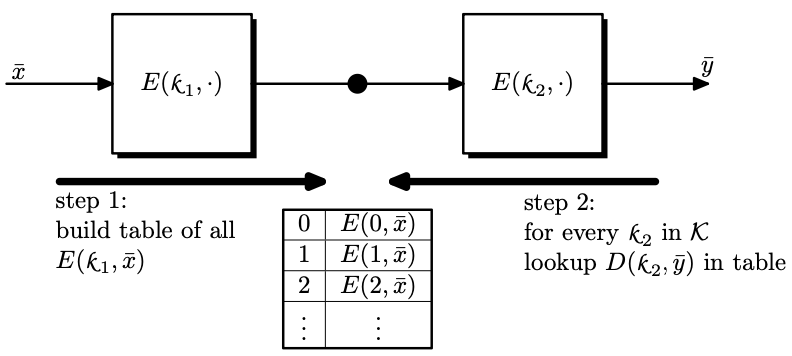
\includegraphics[width=0.6\linewidth]{figures/chapter4/fig10.png}
  \caption{$2\mathcal{E}$上的中间相遇攻击}
  \label{fig:4-10}
\end{figure}

\begin{proof}
令 $\bar{x}:=(x_1,\dots,x_Q)$,$\bar{y}=(y_1,\dots,y_Q)$。为了简化符号,我们用:
\[
\bar y=E_2\big((\mathpzc{k}_1,\mathpzc{k}_2),\;\bar x)=E(\mathpzc{k}_2,\;E(\mathpzc{k}_1,\bar x)\big)
\]
来描述式 \ref{eq:4-9} 中的 $Q$ 个映射。我们也可以把它写成:
\begin{equation}\label{eq:4-10}
D(\mathpzc{k}_2,\bar y)=E(\mathpzc{k}_1,\bar x)
\end{equation}
为了找到能满足式 \ref{eq:4-10} 的一对 $(\mathpzc{k}_1,\mathpzc{k}_2)$,算法 $\mathcal{A}_{{\rm E}X}$ 进行以下操作:

\vspace*{5pt}

\hspace*{5pt} 步骤 $1$:对于所有的 $\mathpzc{k}_1\in\mathcal{K}$,构建一张包含所有数对 $\big(\mathpzc{k}_1,\;E(\mathpzc{k}_1,\bar x)\big)$ 的表 $T$\\
\hspace*{26pt} 步骤 $2$:对于所有的 $\mathpzc{k}_2\in\mathcal{K}$,如下操作:\\
\hspace*{80pt} 计算 $\bar x\leftarrow D(\mathpzc{k}_2,\bar y)$\\
\hspace*{80pt} 查表:如果 $T$ 中包含数对 $(\cdot,\bar x)$,则\\
\hspace*{112pt} 令 $(\mathpzc{k}_1,\bar x)$ 为该数对,输出 $(\mathpzc{k}_1,\mathpzc{k}_2)$ 并停机

\vspace*{5pt}

\noindent
图 \ref{fig:4-10} 描述了这种中间相遇攻击。根据构造,算法输出的数对 $(\mathpzc{k}_1,\mathpzc{k}_2)$ 必然满足式 \ref{eq:4-10},如定理所要求的那样。

算法 $\mathcal{A}_{{\rm E}X}$ 的步骤 $1$ 需要进行 $Q\cdot|\mathcal{K}|$ 次对 $E$ 的评估,而步骤 $2$ 需要进行 $Q\cdot|\mathcal{K}|$ 次对 $D$ 的评估。因此,该算法的全部运行时间就大约是 $2Q\cdot|\mathcal{K}|$ 次对 $E$ 或 $D$ 进行评估的时间。我们假设向查找表 $T$ 中插入元素和查找元素的时间小于评估算法 $E$ 和 $D$ 的时间。
\end{proof}

如上所述,对于相对较小的 $Q$ 值,绝大多数情况下只有一个密钥对 $(\mathpzc{k}_1,\mathpzc{k}_2)$ 满足式 \ref{eq:4-9},它就是定理 \ref{theo:4-2} 中算法 $\mathcal{A}_{{\rm E}X}$ 的输出。

定理 \ref{theo:4-2} 中算法 $\mathcal{A}_{{\rm E}X}$ 的运行时间与对 $\mathcal{E}$ 进行穷举搜索攻击的时间差不多,这表明 $2\mathcal{E}$ 并没有增强 $\mathcal{E}$ 对穷举搜索的抵抗力。然而,该定理只考虑了 $\mathcal{A}_{{\rm E}X}$ 的运行时间。需要注意的是,$\mathcal{A}_{{\rm E}X}$ 必须在内存中维护一张很大的查找表,这可能是很困难的。为了攻击 Double-DES,$\mathcal{A}_{{\rm E}X}$ 需要存储一张规模为 $2^{56}$ 的表,其中每个表项包含一个 DES 密钥和一条短的密文。总的来说,这相当于至少 $2^{60}$ 字节,也就是大约一百万 TB。虽然不是不可能,但获得如此多的存储可能是相当困难的。但是,攻击者可以通过时空权衡的方式来减少存储上的要求,方法是修改 $\mathcal{A}_{{\rm E}X}$,使其在运行过程中仅保留查找表中的 ${1}/{\epsilon}$,代价是运行时间也要相应增加 ${1}/{\epsilon}$。


\begin{snote}[Triple-DES 上的中间相遇攻击。]
类似的中间相遇攻击也适用于上一小节中的 $3\mathcal{E}$ 构造。虽然 $3\mathcal{E}$ 的密钥空间为 $\mathcal{K}^3$,但对 $3\mathcal{E}$ 的中间相遇攻击的时间大约为 $|\mathcal{K}|^2$,所需空间为 $|\mathcal{K}|$。在 Triple-DES 的情况下,该攻击需要对 DES 进行大约 $|\mathcal{K}|^2=2^{112}$ 次评估,这在实践中的运行时间实在太长了。因此,Triple-DES 可以抵御这种中间相遇攻击,这也是 Triple-DES 在实践中能够被广泛使用的原因。
\end{snote}

\subsection{案例研究:AES}

虽然 Triple-DES 是 NIST 批准的密码,但它有一些明显的缺点。首先,Triple-DES 比 DES 慢三倍,在软件中实现时表现很差。其次,$64$ 比特的分组长度对于一些重要的应用来说还是不够(即第\ref{chap:6}章中的应用)。到 20 世纪 90 年代中期,所有人都在期待一个新的联邦分组密码标准。

\begin{snote}[AES的历程。]
1997 年,NIST 发起了一个关于新的分组密码标准的提案征求,该标准被称为\textbf{高级加密标准 (Advanced Encryption Standard, AES)}。NIST 要求 AES 密码必须在 $128$ 比特分组上运行,并支持 $128$、$192$ 和 $256$ 比特三种密钥长度。截止到 1997 年 9 月,NIST 收到了 15 份提案,其中许多来自美国以外的国家。在举行了两次公开会议讨论这些提案后,NIST 在 1999 年将名单缩小到五个候选者。随后又进行了一轮激烈的密码分析,最终在 2000 年 4 月举行的 AES3 会议上,最后五个团队的代表分别作了发言,论证他们的标准为什么应该被选为 AES。2000 年 10 月,NIST 宣布比利时分组密码 \textbf{Rijndael} 被选为 AES 密码。2001 年 11 月,当 AES 作为 NIST 的标准在 FIPS 197 中公布后,它正式成为了一个官方标准。这结束了长达五年的替换 DES 的标准化过程。

Rijndael 是由比利时的密码学家尤安·达蒙(Joan Daemen) 和文森特·雷曼(Vincent Rijmen)设计的。AES 与原始版本的 Rijndael 密码略有不同。例如,Rijndael 支持大小为 $128$、$192$ 或 $256$ 比特的分组,而 AES 只支持 $128$ 比特的分组。
\end{snote}

\subsubsection{AES 算法}

和许多现实中的分组密码一样,AES 也是一个迭代密码,它将一个简单的轮密码迭代数次。迭代的次数取决于秘钥的长度:

\begin{center}
\begin{tabular}{c|c|c|c}
\begin{tabular}[c]{@{}c@{}}cipher\\ name\end{tabular} &
  \begin{tabular}[c]{@{}c@{}}key-size\\ (bits)\end{tabular} &
  \begin{tabular}[c]{@{}c@{}}block-size\\ (bits)\end{tabular} &
  \begin{tabular}[c]{@{}c@{}}number of\\ rounds\end{tabular} \\ \hline\hline
AES-128 & 128 & 128 & 10 \\
AES-192 & 192 & 128 & 12 \\
AES-256 & 256 & 128 & 14 \\ \hline
\end{tabular}
\end{center}

例如,图 \ref{fig:4-11} 展示了一个包含十轮的 AES-128 密码的结构。这里的 $\Pi_{\rm AES}$ 是 $\{0,1\}^{128}$ 上的一个固定置换(即一个双射),它不依赖于密钥。每轮的最后一步是将本轮密钥与 $\Pi_{\rm AES}$ 的输出进行异或。这样重复 $9$ 次,直至最后一轮使用一个稍加修改的置换 $\hat\Pi_{\rm AES}$。AES 的逆运算可以通过反向运行上面的步骤来完成。之所以只需要简单地反向就可以,是因为AES的每一步都是很容易反向运行的。

遵循图 \ref{fig:4-11} 所示结构的密码被称为\textbf{交替密钥密码 (alternating key cipher)} 或\textbf{迭代艾文-曼苏尔密码 (iterated Even-Mansour cipher)}。如果每轮的置换 $\Pi_{\rm AES}$ 满足某些``理想"假设,这种密码就能够确保安全性。我们会在本章后面的定理 \ref{theo:4-14} 中详细分析这一点。

\begin{figure}
  \centering
  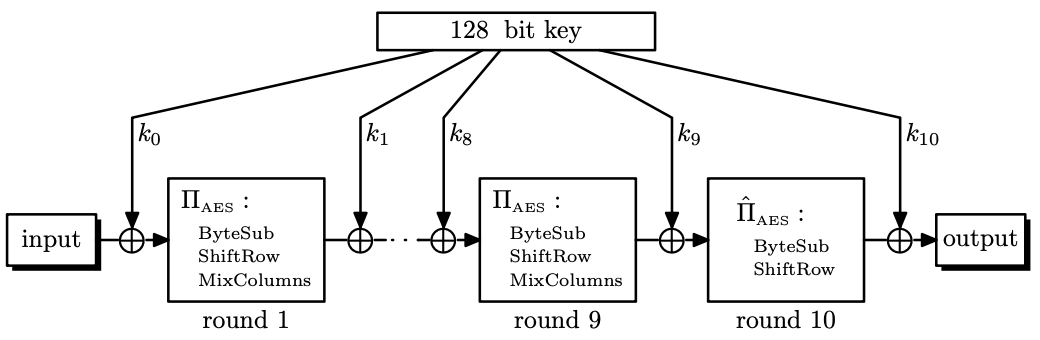
\includegraphics[width=0.7\linewidth]{figures/chapter4/fig11.png}
  \caption{AES-128分组密码的示意图}
  \label{fig:4-11}
\end{figure}

\begin{snote}[AES 轮置换。]
置换 $\Pi_{\rm AES}$ 是由集合 $\{0,1\}^{128}$ 上的三个可逆操作序列组成的。输入的 $128$ 比特会被组织成一个 $4\times4$ 的元胞数组,其中每个元胞是 $8$ 比特。然后,以下三个可逆运算会在这个 $4\times4$ 的数组上依次执行:
\begin{enumerate}
	\item $\mathtt{SubBytes}$:令 $S:\{0,1\}^8\to\{0,1\}^8$ 是一个固定置换(一个双射)。这个置换会被应用于所有 $16$ 个元胞上,一次一个元胞。在 AES 标准中,$S$ 被设计成一个包含 $256$ 个表项的硬编码表。在数学上,$S$ 没有不动点,即对于任意的 $x\in\{0,1\}^8$,$S(x)\neq x$ 都成立。$S$ 也没有拟不动点,即对于任意的 $x\in\{0,1\}^8$,$S(x)\neq \bar x$ 也都成立,其中 $\bar x$ 表示 $x$ 的按位补码。这些要求是抵御 \ref{subsec:4-3-1} 小节中将要讨论的某些攻击所必须的。
	\item $\mathtt{ShiftRows}$:这一步对输入的 $4\times4$ 数组的四行进行按行循环移位:第一行不变,第二行向左循环移动 $1$ 字节,第三行向左循环移动 $2$ 字节,第四行向左循环移动 $3$ 字节。更直观地说,这一步进行了下面这样的转换:
	\begin{equation}\label{eq:4-11}
    \begin{pmatrix}
       a_0 & a_1 & a_2 & a_3\\
       a_4 & a_5 & a_6 & a_7\\
       a_8 & a_9 & a_{10} & a_{11}\\
       a_{12} & a_{13} & a_{14} & a_{15}
    \end{pmatrix}
    \Longrightarrow
    \begin{pmatrix}
       a_0 & a_1 & a_2 & a_3\\
       a_5 & a_6 & a_7 & a_4\\
       a_{10} & a_{11} & a_{8} & a_{9}\\
       a_{15} & a_{12} & a_{13} & a_{14}
    \end{pmatrix}
    \end{equation}
    \item $\mathtt{MixColumns}$:在这一步中,$4\times4$ 数组被视为一个矩阵,该矩阵会与一个固定的矩阵相乘,其中的算术是有限域 ${\rm GF}(2^8)$ 上的运算。有限域 ${\rm GF}(2^8)$ 中的元素可以表示成 ${\rm GF}(2)$ 中元素的不大于 $8$ 阶的多项式,其中的乘法以既约多项式 $x^8+x^4+x^3+x+1$ 为模。具体来说,$\mathtt{MixColumns}$ 的变换是这样的:
    \begin{equation}\label{eq:4-12}
    	\begin{pmatrix}	
    		02 & 03 & 01 & 01\\
    		01 & 02 & 03 & 01\\
    		01 & 01 & 02 & 03\\
    		03 & 01 & 01 & 02
    	\end{pmatrix}
    	\times
    	\begin{pmatrix}
    		a_0 & a_1 & a_2 & a_3\\
    		a_5 & a_6 & a_7 & a_4\\
    		a_{10} & a_{11} & a_{8} & a_{9}\\
    		a_{15} & a_{12} & a_{13} & a_{14}
    	\end{pmatrix}
    	\Longrightarrow
    	\begin{pmatrix}
    		a_0' & a_1' & a_2' & a_3'\\
    		a_4' & a_5' & a_6' & a_7'\\
    		a_8' & a_9' & a_{10}' & a_{11}'\\
    		a_{12}' & a_{13}' & a_{14}' & a_{15}'
    	\end{pmatrix}
    \end{equation}
    这里,标量 $01,02,03$ 被解释为 ${\rm GF}(2^8)$ 上的元素,并用它们的二进制表示(比如说,$03$ 代表 ${\rm GF}(2^8)$ 上的元素 $x+1$)。这个固定矩阵在 ${\rm GF}(2^8)$ 上是可逆的,所以整个变换也是可逆的。
\end{enumerate}

图 \ref{fig:4-11} 所示的 AES 电路中使用的置换 $\Pi_{\rm AES}$ 就由 $\mathtt{SubBytes}$、$\mathtt{ShiftRows}$ 和 $\mathtt{MixColumns}$ 这三个置换按顺序排列而成。在最后一轮,AES 会使用一个稍微不同的函数,我们称之为 $\hat\Pi_{\rm AES}$。这个函数大体上与 $\Pi_{\rm AES}$ 相同,只是省略了 $\mathtt{MixColumns}$ 这一步骤,这是为了使 AES 的解密电路看起来与 AES 的加密电路类似。

因为 $\Pi_{\rm AES}$ 的每一步都是容易逆运算的,所以整个 $\Pi_{\rm AES}$ 置换的全过程也容易逆运算,这也是解密所需要的。
\end{snote}

\begin{snote}[使用预计算表实现 AES。]
AES 的轮函数是由我们之前介绍的置换 $\Pi_{\rm AES}$ 构建的,它包含 $\mathtt{SubBytes}$、$\mathtt{ShiftRows}$ 和 $\mathtt{MixColumns}$ 这三个步骤。但是 AES 的设计者并不是按照这种方式实现 $\Pi_{\rm AES}$ 的,他们提出了一种更高效的方式,能够利用四个固定的查找表 $T_0,T_1,T_2,T_3$ 一次性地完成上面的三个步骤。

为了解释其工作原理,回顾一下 $\Pi_{\rm AES}$ 将一个 $4\times4$ 的矩阵 $A=(a_i)_{i=0,\dots,15}$ 作为输入,并输出一个尺寸相同的矩阵 $A'=\Pi_{\rm AES}(A)$。令 $S[a]$ 为对输入的 $a\in\{0,1\}^8$ 进行 $\mathtt{SubBytes}$ 运算后的结果。类似地,回顾一下 $\mathtt{MixColumns}$ 将当前状态乘以一个固定的 $4\times4$ 矩阵 $M$。令 $M[i]$ 表示 $M$ 的第 $i$ 列,$A'[i]$ 表示 $A'$ 的第 $i$ 列。

现在看一下式 \ref{eq:4-12},我们可以把 $\Pi_{\rm AES}(A)$ 输出的四列表示为:
\begin{equation}\label{eq:4-13}
	\begin{aligned}
		A'[0] & = M[0]\cdot S[a_0]+M[1]\cdot S[a_5]+M[2]\cdot S[a_{10}]+M[3]\cdot S[a_{15}]\\ 
		A'[1] & = M[0]\cdot S[a_1]+M[1]\cdot S[a_6]+M[2]\cdot S[a_{11}]+M[3]\cdot S[a_{12}]\\ 
		A'[2] & = M[0]\cdot S[a_2]+M[1]\cdot S[a_7]+M[2]\cdot S[a_8]+M[3]\cdot S[a_{13}] \\ 
		A'[3] & = M[0]\cdot S[a_3]+M[1]\cdot S[a_4]+M[2]\cdot S[a_9]+M[3]\cdot S[a_{14}]
	\end{aligned}
\end{equation}
其中的加法和乘法都是在域 ${\rm GF}(2^8)$ 上进行的。每一列 $M[i]$ 都是 ${\rm GF}(2^8)$ 上的一个 $4$ 字节向量,而 $S[a_i]$ 是 ${\rm GF}(2^8)$ 上的 $1$ 字节标量。

式 \ref{eq:4-13} 中的每一项都可以用一张固定的预计算表来快速评估。对于 $i=0,1,2,3$,我们定义一张有 $256$ 项的表 $T_i$ 如下:
\[
\text{for }a\in\{0,1\}^8:\quad\quad
T_i[a]:=M[i]\cdot S[a]\quad\in\{0,1\}^{32}
\]
将这些表格接入式 \ref{eq:4-13} 中,就可以得到一个快速计算 $\Pi_{\rm AES}(A)$ 的方法:
\[
\begin{aligned}
A'[0] & = T_0[a_0]+T_1[a_5]+T_2[a_{10}]+T_3[a_{15}]\\
A'[1] & = T_0[a_1]+T_1[a_6]+T_2[a_{11}]+T_3[a_{12}]\\
A'[2] & = T_0[a_2]+T_1[a_7]+T_2[a_8]+T_3[a_{13}]\\
A'[3] & = T_0[a_3]+T_1[a_4]+T_2[a_9]+T_3[a_{14}]
\end{aligned}
\]
以这种方式实现的 AES 电路就是一个简单的查表序列。由于每张 $T_i$ 表中包含 $256$ 个表项,每个表项大小为 $4$ 字节,所以四张表的总大小也不过 4 KB。$M$ 矩阵的循环结构使我们可以进一步将四张表压缩到 2KB,而不对性能产生大的影响。

式 \ref{eq:4-13} 的一个例外是 AES 的最后一轮,这一轮中的 $\mathtt{MixColumns}$ 步骤被省略了。为了计算最后一轮,我们需要第五张 $256$ 字节的表 $S$,它只包含 $\mathtt{SubBytes}$ 的操作。

这个 AES 优化并不是必须的。如果环境极度受限以至于没有足够的空间存储 4 KB 的查找表,你也可以直接按照基本原理用代码分别实现 $\Pi_{\rm AES}$ 的三个步骤,这节约了存储空间,但运算速度可能会慢一点。因此,AES 可以同时适用于有算力约束和算力不受限的环境。

必须要注意的是,这种查表优化的 AES 实现很可能会受到缓存定时攻击,我们将在 \ref{subsec:4-3-2} 小节中介绍这种攻击。
\end{snote}


\begin{snote}[AES-128 的密钥扩展方法。]
回顾图 \ref{fig:4-11},我们看到 AES-128 的密钥扩展算法需要生成 $11$ 个轮密钥 $k_0,\dots,k_{10}$,其中每个轮密钥都是 $128$ 比特。为此,$128$ 比特的 AES 密钥会被分割成四个 $32$ 比特长的字 $w_{0,0},w_{0,1},w_{0,2},w_{0,3}$,这些字构成了第一个轮密钥 $k_0$。其余 $10$ 个轮回密钥按以下顺序产生:对于 $i=1,\dots,10$,$128$比特的轮密钥 $k_i=(w_{i,0},w_{i,1},w_{i,2},w_{i,3})$ 由上一个轮密钥 $k_{i-1}=(w_{i-1,0},w_{i-1,1},w_{i-1,2},w_{i-1,3})$ 产生,方式如下:
 
\vspace*{5pt}

\hspace*{5pt} $w_{i,0}\leftarrow w_{i-1,0}\oplus g_i(w_{i-1,3})$\\
\hspace*{26pt} $w_{i,1}\leftarrow w_{i-1,1}\oplus w_{i,0}$\\
\hspace*{26pt} $w_{i,2}\leftarrow w_{i-1,2}\oplus w_{i,1}$\\
\hspace*{26pt} $w_{i,3}\leftarrow w_{i-1,3}\oplus w_{i,2}$

\vspace*{5pt}

\noindent
这里的函数 $g_i:\{0,1\}^{32}\to\{0,1\}^{32}$ 是 AES 标准中规定的一个固定函数。它对 $4$ 字节输入进行以下三步操作:
(1) 对 $4$ 字节输入进行 $1$ 字节循环左移,
(2) 对得到的 $4$ 字节中的每个字节分别计算 $\mathtt{SubBytes}$,然后
(3) 将最左边的字节与一个固定的轮常数 $c_i$ 进行异或。
轮常数 $c_1,\dots,c_{10}$ 也是在 AES 标准中规定的,其中 $c_i$ 就是 ${\rm GF}(2^8)$ 上的元素 $x^{i-1}$,它被当作一个八比特序列处理。

AES-192 和 AES-256 的密钥扩展方法与 AES-128 的类似。对于 AES-192 来说,每次迭代都会产生 $6$ 个 $32$ 比特的字(共$192$比特),但只有前 $4$ 个字(共$128$比特)会被用作 AES 的轮密钥。对于 AES-256,每次迭代产生 $8$ 个$32$ 比特的字(共$256$比特),也只有前 $4$ 个字(共$128$比特)会被用作 AES 的轮密钥。

AES 的密钥扩展方法被有意设计成可逆的:只要给定最后一轮的密钥,我们就可以反过来恢复完整的 AES 秘钥 $k$。这样做的原因是为了确保每个 AES-128 的轮密钥,就其本身而言,具有与 AES-128 的秘钥 $k$ 相同的熵。不幸的是,可逆性也有助于攻击,它可以被用来发起对 AES 的相关密钥攻击和边信道攻击,我们将在之后讨论这些攻击。
\end{snote}

\begin{snote}[AES的安全性。]
AES 算法经受住了针对它的各种复杂的密码分析尝试。截止到成稿时,最有名的攻击有如下这些:
\begin{itemize}
	\item \textbf{密钥恢复}。密钥恢复攻击是指对手在得到若干明文/密文对的情况下,使用如穷举搜索攻击等方式从这些明密文对中恢复密钥的攻击方式。已知最好的对 AES-128 的密钥恢复攻击需要进行 $2^{126.1}$ 次 AES 计算。这比穷举搜索要快四倍左右,但需要的时间仍然太长了。因此这种攻击对 AES-128 的安全性威胁不大。
	对 AES-192 最好的攻击需要进行 $2^{189.74}$ 次 AES 计算,这也只比穷举搜索快了四倍左右。对 AES-256 的最著名的攻击需要 $2^{254.42}$ 次 AES 计算,这比穷举搜索快三倍。这些攻击都不能影响任何一个 AES 变体的安全性。
	\item \textbf{相关密钥攻击(related key attack)}。在 $\ell$ 路相关密钥攻击中,对手得到了 $\ell$ 张明文/密文对的列表:对于 $i=1,\dots,\ell$,第 $i$ 张表是用密钥 $k_i$ 生成的。重点是,所有 $\ell$ 个密钥 $k_1,\dots,k_\ell$ 都必须满足对手选择的一些固定关系。攻击者的目标是恢复其中一个密钥,比如说 $k_1$。在实现良好的密码系统中,密钥总是独立随机生成的,因此不太可能满足攻击者所需的关系。因此,相关密钥攻击通常不会威胁到正确的加密实现。

    AES-256 容易受到相关密钥攻击,该攻击利用了其相对简单的密钥扩展机制。该攻击需要四个相关密钥 $k_1,k_2,k_3,k_4$,其中的关系是一个简单的异或关系:它要求 $k_1\oplus k_2$,$k_1\oplus k_3$ 和 $k_2\oplus k_4$ 的某些比特被置为特定值。然后给定由这四个密钥产生的明密文对的列表,攻击者可以在 $2^{99.5}$ 时间内恢复这四个密钥。这比在 AES-256 上进行穷举搜索的时间要快得多。虽然这种攻击相当有趣,但它并不能影响 AES-256 在完善的系统中的安全性。
\end{itemize}
\end{snote}

\begin{snote}[AES的硬件实现。]
在 AES 刚被标准化为美国国家加密标准的时候,大多数的实现都还是基于软件的。软件产品对 AES 的广泛采用,促使所有主要的处理器供应商扩展他们的指令集,以增加对 AES 硬件实现的支持。

例如,英特尔在其 Xeon 和 Core 系列处理器中增加了名为 \textbf{AES-NI} 的新指令,以加快在软件中使用 AES 的过程。新指令的工作原理如下:
\begin{itemize}
	\item $\tt{AESKEYGENASSIST}$:运行密钥扩展程序,从 AES 密钥中生成 AES 轮密钥。
	\item $\tt{AESENC}$:运行一轮 AES 轮加密算法。该指令的调用方法是:
	$$
    \tt{AESENC~~xmm15,~~xmm1}
    $$
    其中 $\tt xmm15$ 寄存器保存 $128$ 比特数据分组,$\tt xmm1$ 寄存器保存该轮的 $128$ 比特轮密钥。得到的 $128$ 比特分组会被写入寄存器 $\tt xmm15$。在 AES 的前九轮中,可以事先将轮密钥加载到寄存器 $\tt{xmm1,\dots,xmm9}$ 中,然后调用九次该指令。
    \item $\tt AESENCLAST$:调用与 $\tt AESENC$ 类似的指令来运行 AES 算法的最后一轮。回顾一下,AES 最后一轮的功能与前面几轮稍有不同,它省略了 $\tt MixColumns$ 这一步。
    \item $\tt AESDEC$ 和 $\tt AESDECLAST$:运行 AES 解密算法,与加密指令类似。
\end{itemize}
这些 AES-NI 硬件指令的速度比极尽所能去优化 AES 的软件实现还要更快。艾米利亚·卡斯帕(Emilia Käsper)在 2009 年的实验表明,在英特尔 Core 2 处理器上,使用 AES-NI 指令的 AES 需要 $1.35$ 周期/字节(流水线化),而优化的软件实现则需要 $7.59$ 周期/字节。

在英特尔 2015 年推出的 Skylake 处理器中,$\tt AESENC$、$\tt AESDEC$ 和 $\tt AESENCLAST$ 指令各需要四个周期来完成。这些指令是完全流水线式的,因此每个周期都可以发射一条新指令。换句话说,英特尔将 $\tt AESENC$ 的执行划分为四个阶段的流水线,四个 AES 分组可以由流水线的不同阶段同时处理。虽然处理一个 AES-128 分组需要(4 个周期)$\times$(10 轮)$=$($40$ 个周期)($2.5$ 周期/字节),但在一条流水线上处理四个分组只需要 $44$ 个周期($0.69$ 周期/字节)。因此,流水线可以将 AES 的速度提高近 $4$ 倍。正如我们将在下一章看到的,这在选择我们用来加密长消息的确切方法时起到了重要的作用:选择一种能尽可能地利用并行性来保持流水线繁忙的加密方法是最理想的。

除了速度之外,AES 的硬件实现还提供了更好的安全性,因为它可以抵御下一节中将介绍的边信道攻击。
\end{snote}